\chapter{Methoden}\label{ch:method}



\section{(Statistsiches Verfahren) ABT / Voranalyse}
Mit Hilfe einer sogenantnen Analytical Base Table ist es möglich erste Aussagen über die Datenqualität der zu prüfenden Daten zu treffen.
Zunächst wird diese generiert, um festzustellen, ob die Daten für weitere Untersuchen verwendet werden können.
Anschließend kann ein Plan entwickelt werden, der darstellt, welche Maßnahmen bei unterschiedlichen Datenqualitätsproblemen getroffen werden kann.


\section{Statistische Verfahren für textuelle Attribute}
\label{sec:textVerfahren}
Zur Verbesserung von Texten sind bereits einige Verfahren bekannt, die sich ohne manuellen Aufwand umsetzen lassen.
Eines dieses Verfahren ist die Berechnung der Rechtschreibfehler in den Daten, die als Texte gespeichert sind. 
Solche Fehler entstehen beispielsweise durch die Verwendung von Freitextfeldern in IT-Systemen.  
Einige der in \cite{kiefer2019} vorgestellten Methoden zur Analyse von Datenqualität in Textdaten können auch in diesem Projekt angewendet werden. 
Dazu zählt neben der oben genannten Rechtschreibfehlerberechnung auch der Anteil der unbekannten Wörter. 
Die anderen vorgestellten Verfahren können nicht angewendet werden, da diese sich auf den Kontext von Wörtern oder auf Sätze beziehen und die textuellen Daten in diesem Projekt lediglich zusammenhangslose Wörter sind.
%TODO so lassen:? 
In zukünftigen Projekten, in denen Daten mit Sätzen analysiert werden, sollten die Verfahren, die nur mit Sätzen möglich sind auch in Betracht gezogen werden. \\

Die Autoren schlagen als Tool zur Berechnung der Fehler pyenchant vor. \cite{https://pypi.org/project/pyenchant/}
Pyenchant verwendet unter Anderem Hunspell,\cite{https://abiword.github.io/enchant/} das für bekannte Software, wie z.B. LibreOffice und Firefox zur Rechtschreibkorrektur eingesetzt wird. \cite{http://hunspell.github.io/}
In den Experimenten wird dieses Verfahren praktisch umgesetzt und dessen Ergebnisse dargestellt. 
Der Vorteil einer solchen Berechnung ist, dass nicht nur die Fehler aufgezeigt werden können, sondern auch erkannt wird, welche Daten die Fehler beinhalten. 
Diese können dann an die Stakeholder gegeben werden, um nachgebessert zu werden.
Zukünftig könnten solche Texte auch automatisch mit einer Rechtschreibkorrektur verbessert werden \cite{kiefer2019} \\

Der Anteil der unbekannten Wörter ist ein weiteres Indiz für eine schlechte Datenqualität. \cite{kiefer2019}
Sobald mit diesen Daten Texte analysiert werden sollen, ist dieser Aspekt von besonderer Bedeutung.    Dies gelingt nur, wenn die Verfahren zur automatischen Texterkennung und Analyse die Texte verstehen bzw. interpretieren können. 
Wörter, die zwar nach pyenchant keinen Rechtschreibfehler beinhalten, könnten von einer NLP-Bibliothek, wie NLTK trotzdem nicht erkannt werden. 
Zur Berechnung der unbekannten Wörter kann NLTK verwendet werden. \cite{kiefer2019}
NLTK erzeugt dafür eine Eigenschaft, indem die jeweiligen Wörter mit einem 'X' gekennzeichnet werden. \cite{kiefer2019}
In diesem Projekt liegen nur textuelle Daten zu den Berufen vor, die nicht aufgrund der Anonymisierung unlesbar sind. 
Da eine solche Aussage nur für Texte sinnvoll ist, die in vollständigen Sätzen vorliegen, wird dieses Verfahren in den Experimenten nicht genauer erläutert. 
In zukünftigen Projekten, die sich mit Texten beschäftigen, die von Nutzern geschrieben wurden, ist diese Methode sinnvoll, um Texte analysierbar und nutzbar für die Stakeholder zu machen. 



%Nach \cite{pipino2002} besteht die Schwierigkeit nicht darin die Metriken zu formulieren, sondern die Datenqualitätsdimension zu definieren, die auf den spezifischen Anwendungsbereich des Unternehmens passt. 

%Evtl. kann hier doch noch die Simple Ratio verwendet werden, um die Anzahl der falschen Daten, die das ML errechnet anzuzeigen.%



\section{Machine Learning}
Im folgenden Kapitel werden die Verfahren vorgestellt und kurz beschrieben, die für eine Klassifikation benötigt werden. 
Als Beispiel dient der Risikoscore, da dieser feste Ausgangswerte besitzt und anhand von mehreren Eigenschaften bestimmt wird. 
Mit Hilfe von Machine Learning können die Risikoscores berechnet werden, ohne den Algorithmus zu kennen, der dahinter steckt. 
Dies ist interessant für dieses Projekt, da die Risikoscores bisher bei einer Auskunftei eingekauft werden.
Mit Hilfe eines trainierten Klassifikators können die Daten neu angefordert werden, die sich anhand der Ergebnisse der Klassifikation ändern müssten. 
\\
Ein weiterer Ansatz besteht darin mit Hilfe von unüberwachtem Lernen mögliche Fehler in den Daten zu erkennen.
Anschließend können die als ungewöhnlich markierten Datensätze einem Stakeholder vorgelegt werden.
Nach dem der Stakeholder die Daten zugeordnet hat, die tatsächlich einem Fehler entsprechen, kann mit diesen Labels ein neuer Klassifikator trainiert werden. 
Da dieses Verfahren allerdings sehr viel manuellen Aufwand benötigt und bei diesem Vorgehen Filter wesentlich zuverlässiger verwendet werden können, wird dieser Ansatz nicht weiter verfolgt.
Allerdings ist dies eine gängige Praxis bei Machine-Learning Data Quality tools, wie z. B. talend. 


\subsection{Risikoscoring}
Der Risikoscore wird in dem vorliegendem Unternehmen durch einen externen Dienstleister, eine Auskunftei berechnet. 
Der Dienstleister erhält einige Daten über eine Schnittstelle und anschließend werden diese einem Risikoscore zugeordnet und dem Unternehmen zurückgesendet.
%Des weiteren können Bankmitarbeiter den errechneten Score auch überschreiben und somit einen Einfluss auf die Werte nehmen
Dieser Risikoscore kann mit Hilfe von Machine Learning Methoden berechnet werden, um zu überprüfen, welche Daten aktualisiert werden sollten.
Bei den Daten, bei denen der Wert Abweichungen aufweist können neue Daten angefordert werden.
Dies verbessert die Dimensionen der Richtigkeit und vor allem der Aktualität, die ein Teilgebiet der Richtigkeit darstellt.
\\
Die Scores, die der Klassifikator erzeugt können nicht ausschließlich als Basis für Entscheidungen verwendet werden und kann deshalb nur dabei helfen zu entscheiden, welche Daten aktualisiert werden sollten.
Dies liegt daran, dass Risikoscores nur mit Hilfe von Regressionen berechnet werden dürfen und nicht mit beispielsweise Neuronalen Netzen.



%Vollständigkeit
%Da das Risikoscoring eine wichtige Entscheidungsgröße für die Banken ist, ist davon auszugehen, dass dieses Feld nie leer ist.
%Falls das Feld doch leer ist, sollten die Daten neu angefordert werden. 


Es müssen feste Gruppen von 1A bis 4E vorhergesagt werden. Deshalb bieten sich Klassifikationsalgorithmen an.
Nachfolgend werden die in den Experimenten verwendeten Klassifikatoren vorgestellt und darauf eingegangen, welche Parameter zur Verbesserung des Klassifikationsergebnisses diese haben.

Des weiteren könnte der Klassifikator auch zur Berechnung des Schufascores herangezogen werden. 


\textbf{Vorgehen} \\
1. Daten extrahieren
2. Klassifikator trainieren 
3. Mit Validierung besten auswählen
4. alte Daten und trainierten Klassifikator benutzen, um zu testen, ob es Abweichungen gibt
5. Veraltete Daten anzeigen -> diese sind nun Grundlage zum neu bestellen

\textbf{KNN} \\
Das Grundprinzip des K-Nearest-Neighbor Klassifikators besteht darin die Distanzen eines neuen Punktes zu allen anderen Punkten zu berechnen, um anschließend diesem einer Klasse zuzuordnen.
Für die Zuordnung der Klassen werden die k-nächsten Punkte verwendet.
Hierbei können verschiedene Distanzmetriken verwendet werden. 
Diese sind zum Beispiel die euklidische Distanz oder die Manhattan Distanz.


\textbf{Support Vector Machine (SVM) (mit Multiklassenerweiterung)} \\
Die Idee der SVM besteht darin eine ideale Trennlinie zwischen zwei Gruppen zu finden. 
Hierfür werden sogenannte Stützvektoren (Support Vectors) berechnet, indem eine mathematische Gleichung gelöst wird.
Die Support Vector Machine ist in ihrer Grundform nur in der Lage Zweiklassen-Probleme zu lösen.
Da es in dem vorliegenden Datensatz allerdings mehrere Klassen gibt, ist es notwendig eine Multiklassenerweiterung zu verwenden.
Dafür wird in der Implementierung von Sklearn One vs One verwendet. 
Bei diesem Verfahren werden Kombinationen gebildet, bei denen jede Klasse im Vergleich zu einer anderen trainiert wird.
Um das Ergebnis einer Vorhersage zu erhalten, wird die gewählt, dessen Summe der einzelnen Vorhersagen am Größten ist. 
\\ 
Zur Berechnung der benötigten Vergleiche kann folgende Formel verwendet werden:\\
(NumClasses * (NumClasses – 1)) / 2


\textbf{logistische Regression} %ordinal logistic regression
Bei diesem Verfahren kann die Wahrscheinlichkeit vorausgesagt werden, welche Ausprägungen von unabhängigen Variablen zu einer abhängigen Variable führen. 
Dies wird über einen Threshhold gelöst, der angibt bei welcher Wahrscheinlichkeit eine bestimmte Klasse vorhergesagt werden soll oder nicht.
In unserem Anwendungsfall hat dies den Vorteil, dass bei unstimmigen Datensätze (Wahrscheinlichkeit ist nicht eindeutig) auch neuangefordert werden könnte. 
Da dieses Verfahren darauf beruht, dass die Datensätze unabhängig voneinander sind, muss zunächst die Abhängigkeit der Variablen berechnet werden.
Dies kann mit Hilfe des Pearson Korreleations Koeffizienten erledigt werden.
%Pearson Correlations coefficient -> Testen ob die Daten unabhängig voneinander sind, nur wenn sie das sind funktioniert Logistische Regresseion gut.

\textbf{Classifikation Tree}
Ein Klassifikationsbaum kann dafür verwendet werden, um Regeln zu generieren, die in ein SQL-Skript umgewandelt werden können.
Dies hätte den Vorteil, dass dieser Klassifikator nur einmal trainiert und verwendet werden müsste.
Anschließend kann das Ergebnis des Klassifikators in ein Skript überführt werden und zukünftig in die bestehende Infrastruktur mitabgelegt werden, ohne dass ein Mitarbeiter Kenntnisse für Python oder Machine Learning benötigt. 
Des Weiteren können die gewonnen Informationen verwendet werden, um herauszufinden, welche Eigenschaften besonders wichtig sind.
Dieses Wissen kann verwendet werden, um die Daten, die einen großen Einfluss auf das Klassifikationsergebnis haben händisch zu überprüfen. 
So kann die Datenqualität verbessert werden, indem speziell die Eigenschaften der Daten überprüft werden, die tatsächlich für ein gutes Ergebnis benötigt werden.


%- Neuronale Netze



\textbf{Skalierung}
Skalierung wird angewendet, um die Wertebereiche der Attribute zu normalisieren. 
Dies ist notwendig, da einige Klassifikatoren den Abstand verwenden, um die Zugehörigkeit eines Datenwertes zu einer Klasse zu berechnen.
Hierfür ist es notwendig, dass jedes Attribut den gleichen Einfluss haben kann und nicht das Ergebnis durch ein Attribut dominiert wird. 
Hierfür werden die Eigenschaften der Daten so verändert, dass alle 

Eine Möglichkeit der Skalierung ist die Standardisierung. 
Bei der Standardisierung werden die Werte von den Daten so skaliert, dass diese eine einheitliche Standardabweichung haben. %https://scikit-learn.org/stable/auto_examples/preprocessing/plot_scaling_importance.html
% Standardization involves rescaling the features such that they have the properties of a standard normal distribution with a mean of zero and a standard deviation of one.

Mit Hilfe der Min/Max-Normierung können Merkmale auf den Wertebereich [0,1] abgebildet werden. 

Standardisierung


%(Min/Max)-Normierung : Abbilden der Merkmale auf den Wertebereich [0,1]


%Für Adressdaten (diese sind Texte mit denen ein ML Verfahren nicht so gut umgehen kann):
%-> verwende GPS Daten, die aus PLZ berechnet wurde, damit die Daten einen Zusammenhang haben (Nähe der GPS Koordinaten)
%https://pypi.org/project/pyGeoDb/

%Da es einige Features gibt, muss evtl. zuerst eine Dimensionsreduktion vorgenommen werden.



\subsection{Lösungsansätze für den unbalancierten Datensatz}
In der Verteilung der Daten ist zu erkennen, dass die Klasse, die vom Modell erkannt werden soll unterschiedlich häufig auftreten. 
Dieses Phänomen nennt sich unbalancierter Datensatz und kann dazu führen, dass der Klassifikator die Klasse, die häufiger vertreten, ist bevorzugt. 
Fernandez beschreibt im Buch \cite{Chapter 2 Foundations on Imbalanced Classification von Fernandez}  zwei Handlungen, die zur Lösung berücksichtigt werden müssen. 

\begin{enumerate}
 \item Die Bewertung des Modells darf nicht nur anhand der Accuracy bewertet werden. Ein Datensatz, bei dem 90\% zu Klasse A gehören, könnte eine Accuracy von 90 \% erreichen, indem dieser alle Datensätze als A klassifiziert. Dies könnte zu dem fatalen Schluss führen, der Klassifikator wäre gut geeignet, obwohl dieser nur 0 \% der Klasse B erkannt hat. Als Lösung bieten sich andere Metriken wie beispielsweise f1-Score, precision, recall und ROC an.  
 \item Die Modelle müssen so trainiert und gewählt werden, dass diese die kleinere Klasse gut erkennen können. Außerdem muss dadurch die Accuracy trotzdem gut bleiben. 
\end{enumerate}  \cite{Chapter 2 Foundations on Imbalanced Classification von Fernandez} 

Um das Problem mit den unbalancierten Datensätzen zu lösen existieren einige Ansätze. 
\cite{Chapter 2 Foundations on Imbalanced Classification von Fernandez} 

In dieser Arbeit werden zwei der vorgeschlagenen Lösungen in den Experimenten genauer untersucht. 
Diese ist zum einen das Under- bzw. Oversampling, das auf Datensatzebene die Klassen neu verteilt, um so die Gewichtung der Klassen zu verbessern. 
Zum anderen wird die Möglichkeit getestet durch Veränderung der Kostenfunktion die Falschklassifikation der weniger vorhandenen Klasse mehr zu bestrafen. 
Dadurch muss das Modell sich besser für die schlechteren Klassen anpassen und erzielt somit bessere Ergebnisse. 
\cite{Chapter 2 Foundations on Imbalanced Classification von Fernandez} 


\textbf{Modellbewertung}
Wie beschrieben reicht die Metrik der Accuracy zur Beurteilung von unbalancierten Problemen nicht aus.
Deshalb werden nachfolgend alternative Metriken beschrieben, die mehr Aufschluss über die generelle Güte des Klassifikators geben. 
Die Bewertungsmechanismen helfen dabei die besten Parameter und den am besten für diesen Anwendungsfall geeigneten Klassifikator zu finden.
Folgende Verfahren werden häufig bei der Bewertung eingesetzt:

\textbf{Accuracy}
Diese Metrik gibt an, wie viele der vorhergesagten Werte richtig sind. %\cite{https://scikit-learn.org/stable/modules/generated/sklearn.metrics.accuracy_score.html#sklearn.metrics.accuracy_score}


\textbf{Precision} \cite{Fundamentals of ML Kapitel 8.4.2.2} \\
Precision ist definiert als: \\
\begin{equation}
 \frac{TP}{(TP+FP)}
\end{equation}
Precision beschreibt den Grad an, wie oft ein Datensatz, der vom Klassifikator als korrekt klassifiziert wird, tatsächlich korrekt ist. 

\textbf{Recall} \\
Recall ist definiert als: \\
\begin{equation}
 \frac{TP}{(TP+FN)}
\end{equation}
Recall gibt an, wie viele der positiven Klassen vom Modell als positiv klassifiziert werden. 


Da in dem vorliegendem Klassifikationsproblem ein Multiklassenproblem herrscht, müssen für diese Precision und Recall mit den Ergebnissen aller Klassen vereint werden. 
Hierfür gibt es mehrere Möglichkeiten. 
%\cite{https://scikit-learn.org/0.15/modules/generated/sklearn.metrics.precision_score.html#sklearn.metrics.precision_score}



- Sensitivity und Specifity
- F-Score
- confusion matrix
- auc - roc curve \\
Da die Confusion Matrix TP, FP, FN und TN angibt ist diese gut geeignet. 
Allerdings ist die Standard Confusion Matrix nur für ein Zweiklassen Problem geeignet und in diesem konkreten Fall wird mit einem Mehrklassenproblem gearbeitet.
Deshalb muss die Confusion Matrix auf ein Mehrklassenproblem erweitert werden.
Diese Multiklassenerweiterung ist in dem verwendeten Framework sklearn implementiert und kann ohne weitere Einstellungen verwendet werden.
%https://stats.stackexchange.com/questions/179835/how-to-build-a-confusion-matrix-for-a-multiclass-classifier

\textbf{Under- bzw. Oversampling}
Des weiteren werden in den Experimenten mit den Techniken des Under- bzw. Oversamplings gearbeitet. 
Diese Verfahren sind in der Lage unbalancierte Datensätze, wie den vorliegende Datensatz, für die Modelle vorzubereiten. 
Dies geschieht beim Undersampling, indem die Daten reduziert werden, sodass alle Klassen die gleiche Verteilung aufweisen. 
Beim Oversampling auf der anderen Seite werden die Daten, die in einer Unterzahl sind durch mehrmaliges einfügen auf die Menge der anderen Klassen gebracht. 
Dies führt dazu, dass in den Daten, Datensätze redundant vorhanden sind. 
Deshalb sollte dieses Verfahren nur auf den Trainingsdaten angewendet werden, da sonst der Klassifikator mit den gleichen Daten trainiert wird, die auch zum Testen verwendet werden. 
Auch das Undersampling sollte nur auf den Trainingsdaten erfolgen, da sonst nicht überprüft wird, wie der Klassifikator in einer realen Anwendung abschneiden würde, in der die reale Verteilung der Daten vorliegt. \cite{ZITAT}
\cite{ML 3.6.3 Sampling}
Der Nachteil des Oversamplings besteht darin, dass die Modelle overfitten, da mehr Datensätze die gleiche Klasse repräsentieren, sie werden also tendenziell bevorzugt. 
\cite{ML 4.4.4 Tree Pruning}
Oversampling wird verwendet, wenn zu wenig Datensätze vorhanden sind und Undersampling, falls genügend viele Daten verfügbar sind. 

\textbf{Modell Anpassung}
Als Alternative zum Sampling können die Modelle stärker bestraft werden, wenn diese falsch klassifizieren. 
Dies führt dazu, dass die Modelle besser generalisieren, da die 

% "Adjusting Class Votes" für Sigmoid und Majority Vote
% Nachfolgender Link zeigt die Verwendung von Class-weights in SVM https://machinelearningmastery.com/cost-sensitive-svm-for-imbalanced-classification/

Holdout
k-Fold
stratified k-Fold

Optimierung von Hyperparametern 
-> Einteilen in Train/Dev/Test

Vergleichen der versch. ROC-Kurven:
ROC / AUC

%TODO Was ist Overfitting

\subsection{Auswirkungen der einzelnen Merkmale auf das Gesamtscoring}
Es ist wichtig zu wissen, wie sich das Scoring zusammensetzt, um gezielt die Daten zu verbessern, die einen großen Einfluss haben. 

Wie groß sind die Auswirkungen der einzelnen Merkmale auf das Gesamtscoring. 

\section{Visualisierung}
Auch mit Hilfe einer Visualisierung können Informationen über die Daten gewonnen werden.
In diesem Projekt werden die Daten visualisiert, die angeben, wie viele Daten extrahiert wurden.
Dies geschieht in Echtzeit und werden anschließend in einem Dashboard dargestellt.
Die Stakeholder können anhand diesem Dashboards sofort erkennen, ob die Datenmenge ungewöhnlich ist im Vergleich zu sonstigen in der Vergangenheit liegenden Datenlieferungen.
Dies ist ein Indiz für Fehler, die in der Programmierung entstanden sind.


\subsection{Data Quality Dashboard / Auswahl des richtigen Tools zur Visualisierung}
% Tableau beschreiben , beispiel
% Grafana, Kibana
% Bewertung von Tablaeu anhand Experten Meinung 
% Eigener Vorschlag / Konzept Visualisierung 

% Befragung des Experten?

Es gibt einige Unternehmen, die Software anbieten, mit denen Visualisierungen und Analysen erstellt werden können. 
Beispielsweise gibt es das Unternehmen Tableau, das eine umfassende Software anbietet, mit der Visualisierungen erstellt, aber auch ETL-Prozesse grafisch entwickelt werden können.  
\cite{https://www.tableau.com/de-de/why-tableau/what-is-tableau}

Auf der Webseite von Tableau ist ein Beispiel für ein Data Quality Dashboard zu sehen. 
Dieses stellt die unterschiedlichen Qualitätsmetriken dar und mit Hilfe einer Ampellogik können Entscheider erkennen, ob die Qualität ihren Vorstellungen entspricht.
Siehe \cite{https://public.tableau.com/views/DataQualityDashboards/Dashboard1?:embed=y&:showVizHome=no&:display_count=y&:display_static_image=y&:bootstrapWhenNotified=true}
Die Stakeholder in dem vorliegenden Projekt haben nach Befragungen erklärt, dass sie ein solches System gesehen haben und sich wünschen. 
Sie erhoffen sich dadurch Aussagen zur Daten Qualität treffen zu können, falls sie Auskunft darüber geben sollen. 
Die Vorteile liegen also nur darin eine Aussage zu treffen nicht aber, um tatsächlich mit dem Ergebnis etwas anzufangen. 
Daraus ergeben sich erst in weiteren Schritten tatsächliche Vorteile, die weitere Voraussetzungen benötigen.
Es ist notwendig einen konkreten Stakeholder zu bestimmen, der für die Einhaltung der Qualität verantwortlich ist.
Ohne eine solche Person können Probleme, die aufgrund schlechter Datenqualität entstehen, nicht behoben werden, da keiner Zeit und Energie in eine Lösung steckt.

Um ein solches Dashboard zu erzeugen müssen einige Vorarbeiten von den Stakeholdern geleistet werden.
Jedes Datenattribut benötigt einen Wertebereich, um eine Aussage darüber treffen zu können, ob ein Attribut innerhalb der geforderten Datenqualitätsdimension liegt oder außerhalb.
Des weiteren muss definiert werden, bei welcher Abweichung ein Attribut als rot, grün bzw. gelb markiert werden sollte. 
In der Grafik von Tableau ist allerdings auch zu erkennen, dass diese 

Insgesamt ist die Aussagekraft eines solchen Dashboards zu hinterfragen. 

Als Erweiterung zu dem dargestellten Dashboard ist eine Drill-Down Funktionalität notwendig.
Mit dieser ist es möglich auf das Datenattribut selbst zuzugreifen. 
Anschließend kann dieses Attribut, wenn klar ist, wo es herkommt und wer es erzeugt hat, ausgebessert werden.
% Von Experten Interview 
An dieser Stelle wäre es nötig die Quelle selbst zu verbessern. % An der Quelle suchen
Es können auch Probleme auftreten, die erst durch den Programmcode der Entwickler entstanden ist.
Hierfür wird nachfolgend eine Möglichkeit dargestellt, um die Extraktionen zu überwachen.
% Fehler in den Daten -> abbruch -> Neustarten -> zurück an Entwicklungsabteilung
% Richtige Anzahl extrahiert (ist gleich viel auf beiden Seiten) (einfaches Group By bzw Rollup)
% 
Als Alternative bietet sich eine Visualisierung mit Kibana oder Grafana an.
Dies sind Tools mit denen auch ein Dashboard dargestellt werden kann.
Im Gegensatz zu Tableau, liefern diese zwar nicht die Funktionalität für ein explizites Data Quality Dashboard, allerdings könnte ein solches nur durch den beschriebenen manuellen Aufwand der Stakeholder, der Definition von Schwellwerten, befüllt werden.
Mit Hilfe der Visualisierungsmöglichkeiten in Grafana und Kibana ist es dennoch möglich Aussagen über die Datenqualität abzuleiten, für die kein manueller Aufwand durch die Stakeholder nötig ist.
Eine dieser Möglichkeiten ist eine Zeitreihenanalyse, mit der die Daten im historischen Kontext betrachtet werden können.
Dazu müssen die Daten in das Tool integriert werden und anschließend mit Hilfe der eingebauten SQL-Engine richtig gruppiert werden.
%Hier noch mehr Argumente finden
Anschließend können anhand der Visualisierung erkannt werden, ob es Tage oder Programme gibt, die besonders viel Zeit benötigen oder ob bestimmte Attribute ungewöhnlich häufig verändert wurden. \\

\textbf{Warum Grafana}
Die beiden Tools Grafana und Kibana sind beide Open-Source und bieten somit eine kostengünstige Variante an, um ein Dashboard zu erstellen. 
Des weiteren bietet Grafana eine Vielzahl von Plugins an, die es ermöglichen die Software einfach zu erweitern, um neue Funktionalität hinzuzufügen. 
Hierfür können auch eigenen Plugins geschrieben werden, wenn diese benötigt werden.

Die Stärken von Kibana liegen allerdings in der Auswertung von Log-Dateien.
Diese Fähigkeiten werden allerdings nicht benötigt, sondern es werden Daten visualisiert, die schon als relationale Daten vorhanden sind. 
Auch die Metadaten der Prozesse werden aus Log-Dateien schon in eine relationale und leicht weiterverarbeitbare Form gebracht. 
Deshalb wäre es nicht sinnvoll die Daten wieder in Log-Dateien zu überführen, wenn die Daten schon in einer Form vorliegen, in der sie gut weiterverarbeitet werden können. 
Grafana bietet zu dem, im Gegensatz zu Kibana, die Möglichkeit die Daten mittels SQL aufzubereiten und zu aggregieren. 
Des weiteren müsste für die Verwendung von Kibana noch zusätzlich Elastic eingerichtet, verwaltet und verwendet werden. 
Falls in Zukunft Daten aus Elasticsearch verwendet werden würde, könnte dies auch in Grafana integriert werden, da die Software auch dafür eine Anbindung anbietet. 

Beispielsweise bietet Grafana eine Vielzahl von Plugins an.

\textbf{Integration der Daten in Grafana} \\
Diese können verwendet werden, um komfortabel Daten anzubinden.
Eine Möglichkeit ist das Plugin CSV, das in der Lage ist Daten aus einer CSV-Datei direkt in Grafana zu verwenden. 
Allerdings ist dieses Plugin noch in einer frühen Entwicklungsphase und wird deshalb nicht in diesem Projekt verwendet. \cite{https://grafana.com/grafana/plugins/marcusolsson-csv-datasource?pg=plugins&plcmt=featured-undefined}
Des weiteren bietet Grafana die Möglichkeit Daten mit Hilfe eines JSON-Formats zu importieren. 

Es sind einige Konnektoren als Plugin für Grafana verfügbar, allerdings fehlt dort die Möglichkeit eine DB2-Datenbank anzubinden. \cite{https://grafana.com/grafana/plugins?type=datasource}
Auch fehlt die Möglichkeit über eine allgemeine JDBC-Verbindung proprietäre Datenbanksysteme anzubinden.


% kostenlos
% einfach anzubinden, da nicht konvertierung in log-Dateien notwendig 
% Umfangreiche Anzeige möglichkeiten von Daten -> Dashboards
% Zeitreihenanalyse für Anomalie Erkennung 


% Preis
% Einfache Integration 
% Anzeige der Daten als Dashboard (erfüllen alle 3)
% Zeitreihenanalye 
% Interaktiv

- Kibana Daten
- Dashboard für Ampel logik

\section{Sicherstellung der korrekten Prozesse}
Ein weiterer wichtiger Aspekt guter Datenqualität besteht darin die Prozesse der Extraktionen so zu gestalten, dass diese fehlerfrei sind.
Für diesen Anwendungsfall wird ein Dashboard erstellt, das live die Metadaten der Prozesse erhält und anschließend visualisiert.
Es bieten sich folgende Visualisierungen an.
Ein Linienchart zur Darstellung des zeitlichen Verlaufs.
Des weiteren ist es gut die mittlere Abweichung der Anzahl der extrahierten Daten mit darzustellen. 
Dadurch ist es möglich zu erkennen, ob ungewöhnlich viele bzw. wenige Daten verarbeitet wurden. 


\begin{figure}[h]
\centering
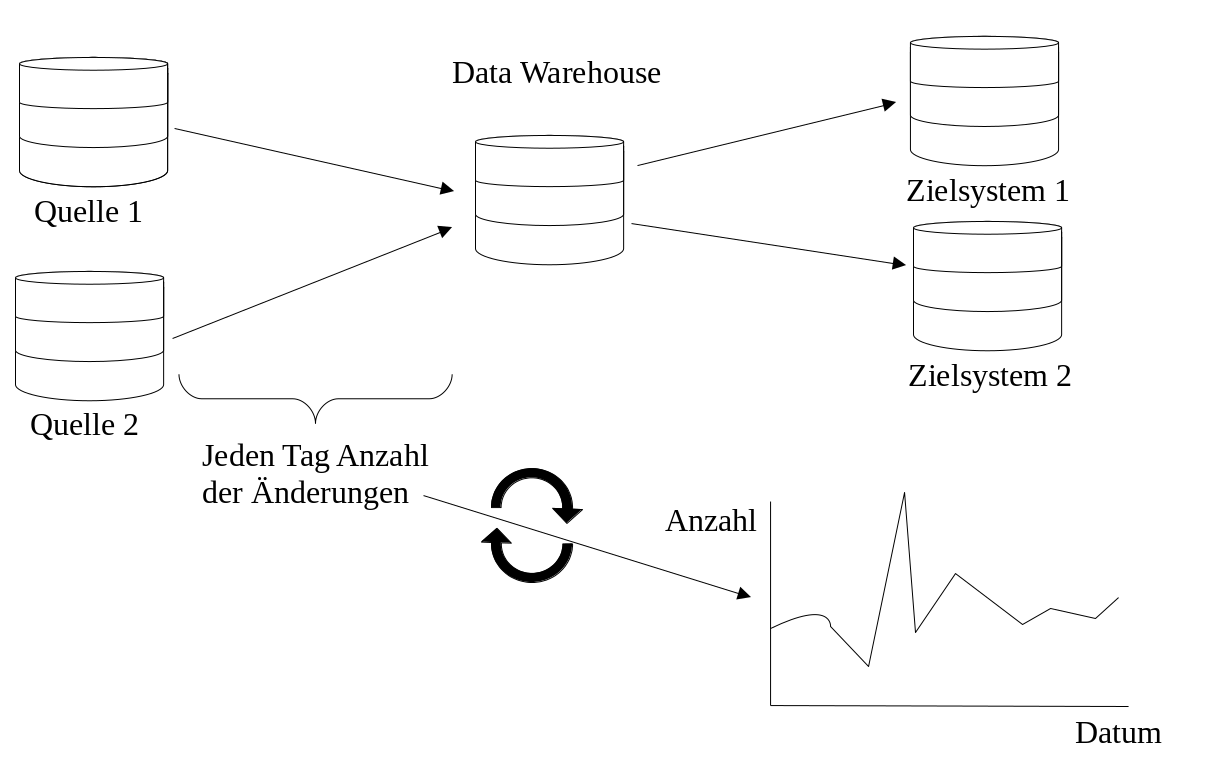
\includegraphics[width=150mm,scale=1]{content/Darstellung_vis_pipeline.png}
\caption{Darstellung des aktuellen Extraktionsverfahrens und Integration der Visualisierung }%
\end{figure}
Die Abbildung zeigt den aktuellen Extraktions-Prozess des Data Warehouse. 
Bei diesem werden Daten aus einigen Quellsystemen abgeholt und in eine zentrale Datenbank, dem Data Warehouse extrahiert.
Anschließend werden die Daten in das korrekte Format konvertiert und den Endsystemen so bereitgestellt, wie diese die Daten erwarten.

Eine mögliche Visualisierung sollte die Meta-Daten, die von den Quellsystemen extrahiert werden erhalten und anschließend visualisieren.
Hierfür wird per Trigger die Daten in Echtzeit an Elastic übertragen, dass die Daten anschließend mit Hilfe eines Kibana Dashboards visualisiert.
Stakeholder sind dann in der Lage grafisch zu sehen, ob es große Abweichungen zu den Monaten / Wochen / Jahren davor gegeben hat und können so einschätzen, ob genauer nachgeforscht werden muss oder ob alles geklappt hat.




%Daten zur Beladung (Delta, Vollbestand) in Echtzeit aus dem DWH nach Elastic exportieren
%-> Anhand eines Dashboards ist es möglich festzustellen, ob es Abweichungen gibt
%-> Ein Experte kann diese Abweichungen dann überprüfen



%Vollständigkeit auf Datensatzebene
%Vollständigkeit auf Attributwerte (es kommen keine null-values hinzu)


%Aktualität die Daten werden schnell genug abgeholt
%Richtigkeit die Daten werden so abgeholt, dass sie fehlerfrei sind

%Ideen:
%- Source und Target vergleichen
%- historisch vergleichen, wie viel zu erwarten ist
%- 

%Die Daten müssen innerhalb einer vorgelegten Range liegen, damit sichergestellt wird, dass die Daten in dem Zielsystem richtig ankommen.



%Zuverlässigkeit, Protokollierung, Dokumentation, Audit der Prozesse
% Verfügbarkeit, Wartbarkeit, Nachvollziehbarkeit







